\documentclass{acm_proc_article-sp}

\begin{document}

\title{Conversing verses - haiku generation using a LSTM-based auto-encoder matching model}

\numberofauthors{2} 
\author{
\alignauthor
Luka Ernestini\\
       \affaddr{Univerza v Mariboru}\\
       \affaddr{Fakulteta za elektrotehniko, računalništvo in informatiko}\\
       \affaddr{Maribor, Slovenija}\\
       \email{luka.ernestini@student.um.si}

\alignauthor
Niko Uremović\\
       \affaddr{Univerza v Mariboru}\\
       \affaddr{Fakulteta za elektrotehniko, računalništvo in informatiko}\\
       \affaddr{Maribor, Slovenija}\\
       \email{niko.uremovic@um.si}
}

\maketitle
\begin{abstract}

\emph{empty beaches / the warmth of our tears / end of summer}

In the field of natural language processing, many methods of deep learning have been developed for text generation. In our paper we explore a novel method for Haiku poetry generation, combining the approaches of generating the first verse using GRU network, with the Auto-Encoder matching model for generating the second and third verse of the Haiku poem as a form of conversation between the verses. By using the Auto-Encoder matching model to generate the second and third verse as an answer to the previous verse, we experiment by adding a sense of conversational bond between the verses. Human evaluators indicated that the generated Haikus were generally of worse quality than human Haikus, except some lucky outliers that were considered so good that they were classified as human made.

\end{abstract}

% todo: kaj to pomeni
\category{H.4}{Information Systems Applications}{Miscellaneous}

% todo: kaj to pomeni
\terms{Theory}

\keywords{text generation, neural networks, LSTM}

\section{Introduction}

Deep learning is an emerging machine learning approach that can already be seen applied in many industries, including natural language processing. Example use cases include identifying people and objects in images and videos, understanding voice commands (smartphones, cars, smart houses) and providing better results for internet search queries. This technology brought machines the closest they have ever been to how we humans think and talk. Having learned the rules and grammar of our natural language, machines are now able to generate text for various applications that is in some cases indistinguishable from human written text \cite{pawade2018story}.

In the field of natural language processing, many methods of deep learning have been developed for text generation. Song, Huang and Ruan \cite{song2019abstractive} achieved Abstractive Text Summarization (ATS) using and LSTM-CNN based ATS framework (ATSDL). You et al. \cite{You_2016_CVPR} researched ways to generate natural language descriptions of images. They proposed a model of semantic attention which combines the established top-down and buttom-up approaches. CNN is used for image classification, followed by LSTM-based RNN for the caption generation. Bhagavatula et al. \cite{bhagavatula2020abductive} investigated the viability of natural language-based abductive reasoning.

One of the obstacles in the field of text generation has been the objective evaluation of the generated text's semantics. While the spelling and grammar correctness are easy to evaluate, the meaning of the generated text can be challenging to evaluate with an automated metric \cite{celikyilmaz2020evaluation}. Some tasks of text generation, such as image captioning or machine translation, where the (suggested) correct generation is known, can use metrics like BLEU \cite{papineni2002bleu} or METEOR \cite{banerjee2005meteor}, to evaluate the quality of the generated text. On the other hand, tasks where the correct generation is not specified (e.g., story \cite{pawade2018story} or poem \cite{zhang2014chinese} generation), the quality of the produced text is usually evaluated by human readers.

We draw inspiration for our research from the work of Luo et al. \cite{luo2018autoencoder}, who propose a novel Auto-Encoder matching model to learn utterance-level semantic dependency for generating everyday dialogue. Three neural networks are used: LSTM for encoding a reply into it's semantical representation, then a feedforward network for mapping the reply semantic into the answer semantic. Lastly a LSTM decoder is used for the sentence generation. Additionally, we found motivation for our work in the success on the field of poem generation by Potash, Romanov and Rumshisky \cite{potash2015ghostwriter}, who demonstrated the generation of rap songs using LSTM, and Netzer et al. \cite{netzer2009gaiku}, who explored the usage of Word Association Norms (WAN) to generate Haiku poetry.

In the paper, we present a novel method for Haiku poetry generation, combining the approaches of generating the first verse using GRU network, with the Auto-Encoder matching model \cite{luo2018autoencoder} for generating the second and third verse of the Haiku poem as a form of conversation between the verses. RNN, such as GRU or LSTM has proven to be capable of mimicking rhythm, common phrases and even poet's writing style \cite{potash2015ghostwriter}, which we attempt to use for generating the text in a genuine Haiku style, which we describe in the continuation of the work. By using the Auto-Encoder matching model to generate the second and third verse as an answer to the previous verse, we experiment by adding a sense of conversational bond between the verses.

\section{Background}

Haiku is a form fo poetry of poetry originated in Japan and later adopted in Western languages. Traditional Haiku consists of three lines with five, seven and five syllables, however this form has been loosened in non-Japanese versions of Haiku. We adopt this loosened form of Haiku, with only syntactic constraint being 3 short verses.

For the training corpus, we selected approximately 17 thousand poems from a larger Haiku dataset, containing over 118 thousand English Haikus. Selected Haikus comply with our loosened syntactic constraint, wereas other poems in the dataset were of more experimental nature (empty or very long verses, unconventional use of punctuation, grammatically flawed).

\section{Methodology}

The proposed methodology of generating Haiku poetry consists of the following steps: generating the first verse of the poem using a GRU-based model, and generating the second and third verse using the modified Auto-Encoder matching model. The poem generating framework thus consists of 5 neural networks of 2 types. First type is the auto-encoder GRU-based network with 2 GRU cells. First GRU cell processes the verse and encodes it in a hidden state, which is then decoded by a second GRU cell that generates the output from the given state. 3 such networks are used in the framework, one for each verse. The second type of the neural network is a mapping network, that transfers the information from one verse to another. The mapping network consists of 2 fully-connected layers. The architecture of the auto-encoder model type is presented in Figure \ref{fig:autoenc}, and the architecture of the mapping module in Figure \ref{fig:mapping}.

\begin{figure}[h!]
	\centering
	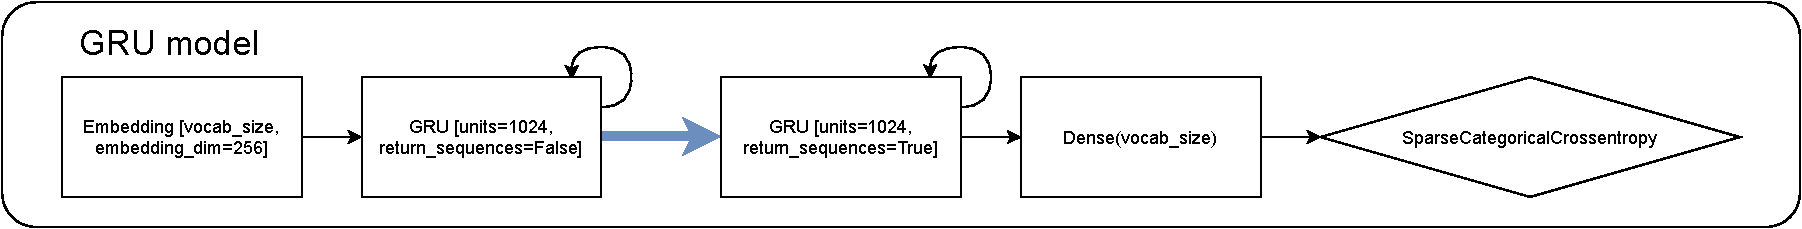
\includegraphics[width=0.45\textwidth]{flowchart/autoenc.pdf}
    \caption[The architecture of the auto-encoder model type.]{The architecture of the auto-encoder model type.}
    \label{fig:autoenc}
\end{figure}

\begin{figure}[h!]
	\centering
	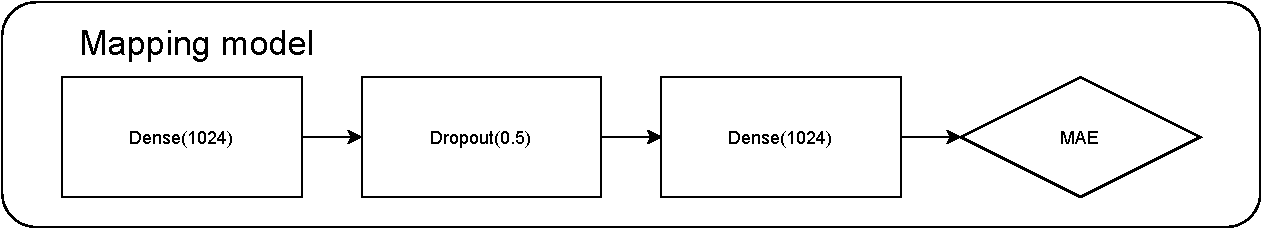
\includegraphics[width=0.45\textwidth]{flowchart/mapping.pdf}
    \caption[The architecture of the mapping module.]{The architecture of the mapping module.}
    \label{fig:mapping}
\end{figure}

The procedure of generating the Haiku with trained models is more precisely presented in the Figure \ref{fig:generation}.

\begin{figure}[h!]
	\centering
	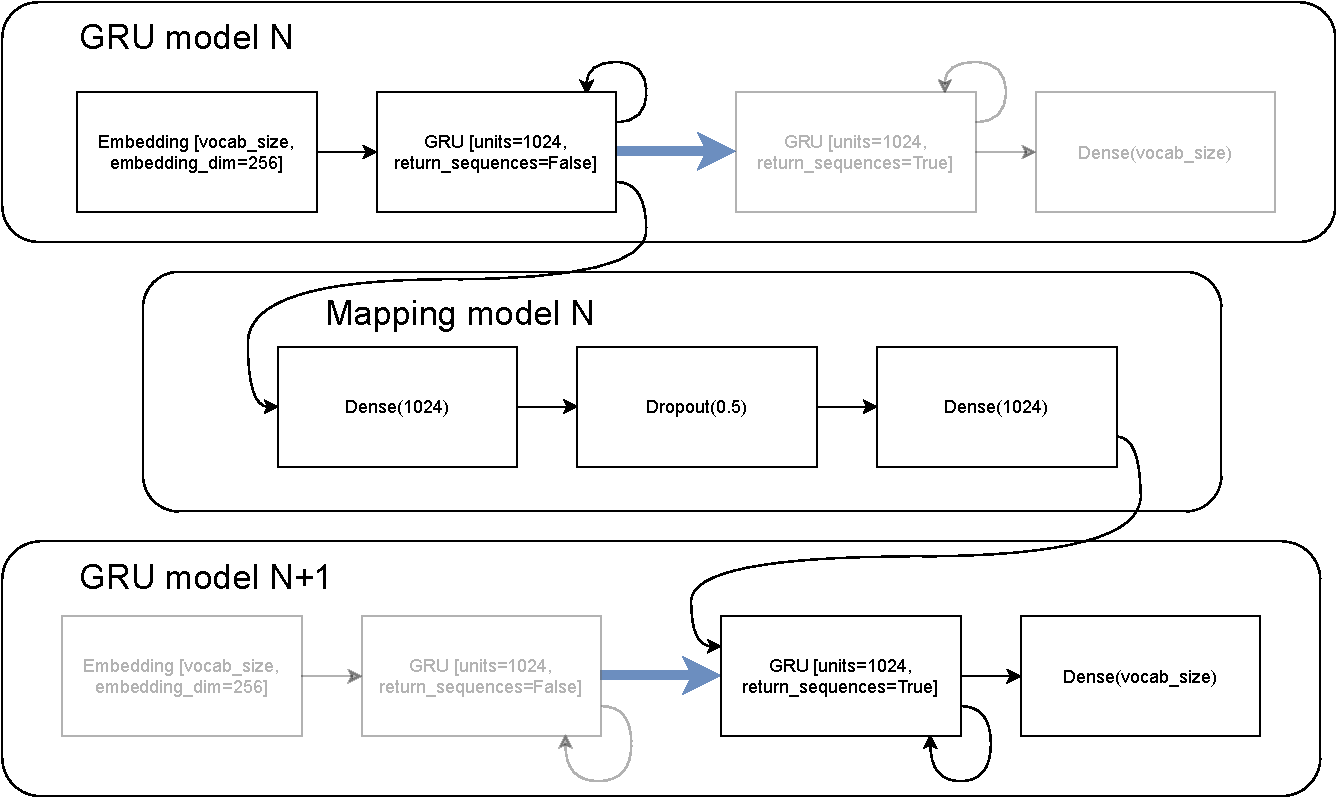
\includegraphics[width=0.45\textwidth]{flowchart/generation.pdf}
    \caption[The procedure of generating the Haiku with trained models.]{The procedure of generating the Haiku with trained models.}
    \label{fig:generation}
\end{figure}

While training the GRU models is fairly straightforward (the auto-encoder model is supposed to generate the same output as the input it was given), the training of a mapping module is somewhat more complicated. Authors \cite{luo2018autoencoder} of auto-encoder matching model for dialogue generation, train the mapping module by passing the encoded hidden state of an auto-encoder into a mapping module, and then decoding the mapped hidden state with auto-encoder and comparing it to the expected output (reply in a conversation). While we could in theory do the same (encode verse 1 with auto-encoder for 1st verse, map the hidden with mapping module 1 and then decode the mapped hidden state with auto-encoder for the 2nd verse, similar for the following 3rd verse), this is a very computationally difficult task. While we could pre-process the encodings of each verse, we would still have to do all the decoding operations with each training step, leading to very long training times. To mitigate this, we propose a simpler approach presented in Figure \ref{fig:training}. Instead of decoding the mapped hidden state, the mapped hidden state itself is compared to an estimation of the expected hidden state. This approach offers significantly faster training times, however the exactness of the approach is not optimal, which we further discuss in the following sections.

\begin{figure}[h!]
	\centering
	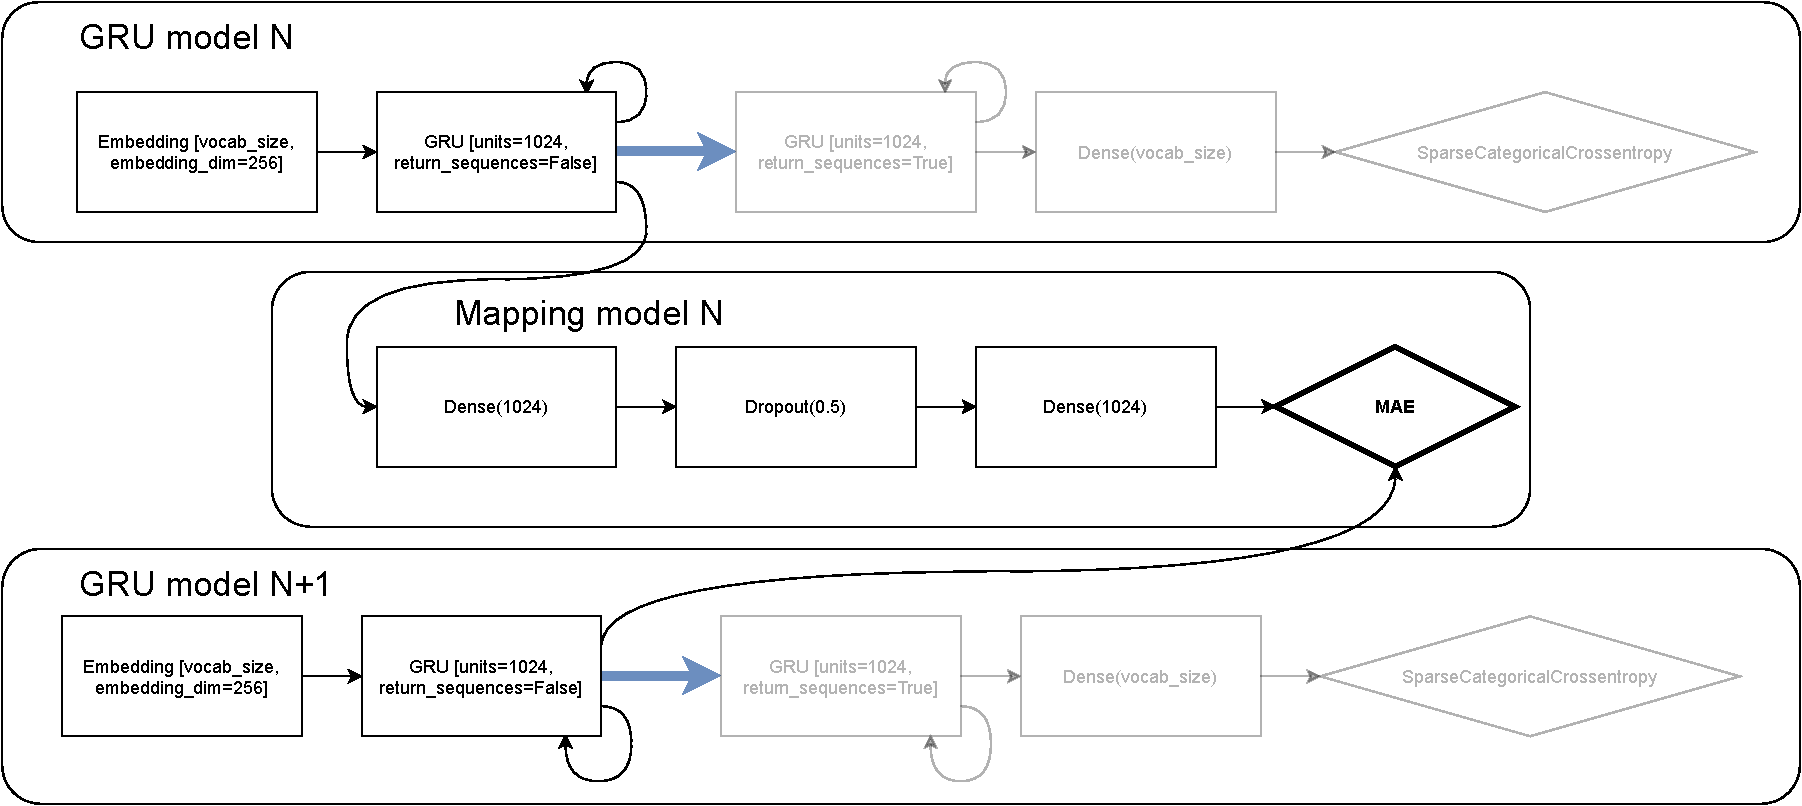
\includegraphics[width=0.45\textwidth]{flowchart/training.pdf}
    \caption[The procedure of training the mapping module.]{The procedure of training the mapping module.}
    \label{fig:training}
\end{figure}

The whole framework is presented in the Figure \ref{fig:fw}.

\begin{figure}[h!]
	\centering
	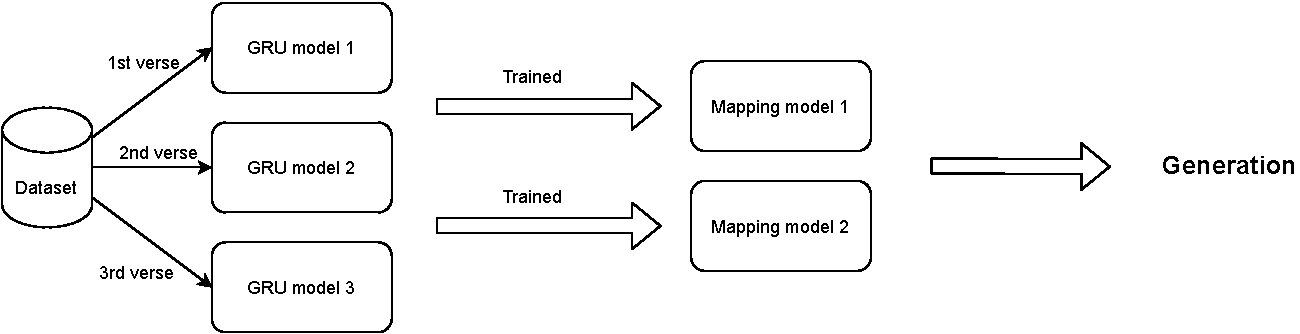
\includegraphics[width=0.45\textwidth]{flowchart/fw.pdf}
    \caption[The Haiku poem generation framework.]{The Haiku poem generation framework.}
    \label{fig:fw}
\end{figure}

\section{Results}

We wanted to compare the efficacy of our approach of generating Haikus with Gaiku \cite{netzer2009gaiku}, so we conducted the evaluation in a similar fashion. We asked some fellow students to read through 20 haiku poems and to assign two ratings to each, on a scale of 1 to 5: how much they like the poem and whether they think it was writen by a human or generated by a computer. Of the 20 Haiku poems, 12 were generated and 8 were selected from our corpus. The subjects did not know the ratio between the two. The questionnaire was answered by 20 subjects and all were fluent in English, but not experts, nor did they have an academic background in literature.

By having our evaluators give two ratings (the poem likeness and how artificial it seems), we were able to see that they were more inclined toward stating that the poem was human-made if they liked it and vice versa. This also means that they felt that a generated haiku poem could not be as good, which led to 3 artificial poems being confidently rated as human-made.

\begin{figure}[h!]
	\centering
	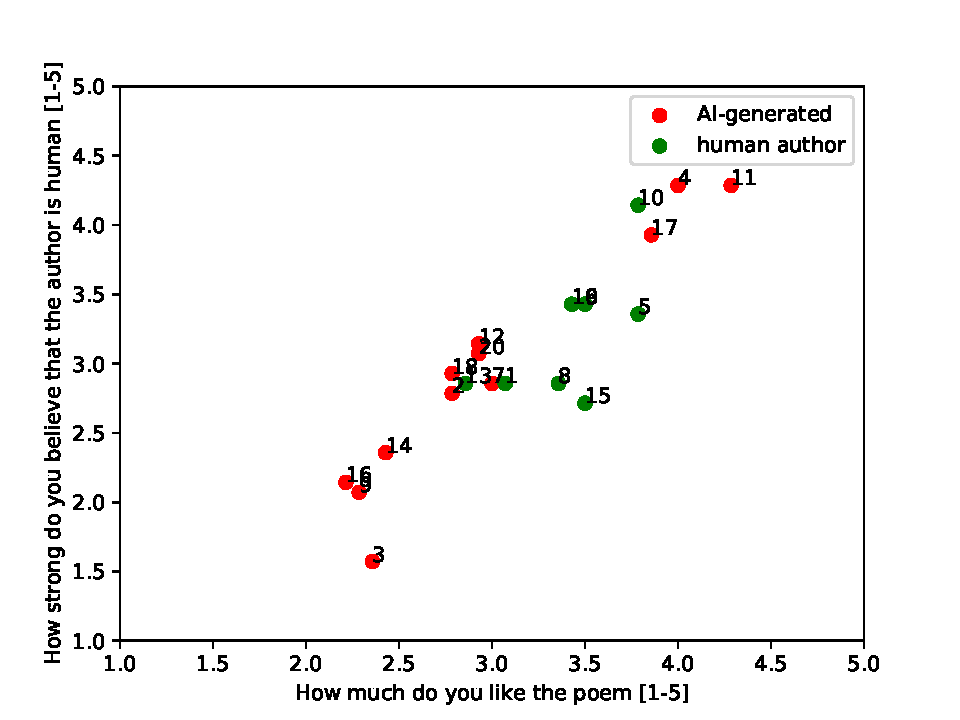
\includegraphics[width=0.45\textwidth]{average_score_poems_2.pdf}
    \caption[The evaluation result.]{The evaluation result.}
    \label{fig:results}
\end{figure}

Of the 8 poems composed by human authors, four were falsely thought to have been artificial, however all were very close to uncertainty (3), with the lowest rating being 2.71. That poem was:

\emph{dusk-- / songbirds' voices / disappear too}

On the other hand, 8 of the 12 computer generated haikus were correctly classified as such.

The poem that was most strongly classified as computer generated, and correctly so, was:

\emph{evening coffee / the chalkboard scent / belly}

with a rating of 1.57, while it's likeness rating was 2.36.

On the other hand, the two haikus most strongly classified as human-made were actually
computer generated. These two were:

\emph{early storm warning / I stand next to a tree / coloured into darkness}

and

\emph{empty beaches / the warmth of our tears / end of summer}

with the latter also having the highest likeness score of all poems at 4.29.

There was, as was expected, a high variance in scoring. This can be attributed to the fact that our evaluators were not experts in the field and to the subjective nature of rating poetry (particularly Haiku). \cite{ritchie2001creativity}Most human poems got an above average rating, while auto-poems got mostly worse, but surprisingly some better ratings too.

\section{Conclusions}

We present a novel method for poem generation, applied to the field of Haiku poems. The method utilizes auto-encoder models based on GRU for learning poem characteristics on verse-basis and a mapping module for propagation of information between the verses. A sample of generated poems were together with a sample of human-written poems presented to a number of respondents, that evaluated both generated and human-written poems. While an average generated poem was evaluated 27\% worse than an average human-written poem, there were 3 outstanding poems generated that were evaluated as good as one of the best human-written poems in the sample presented.

The results could be improved by ommiting the training cost optimization explained in section Methodology. Two factors that make this approach inexact, are the following: simply comparing the mapped multi-dimensional hidden state to so-called "estimated expected hidden state" with metric MAE is far from optimal, since the importance/sensitivity of each element in a hidden state vector is not the same. Secondly, the "estimated expected hidden state" is as the phrasing suggests, just an estimation. There can be a number of hidden states that would decode into a target verse, and finding such sub-space of hidden states (if it even exists - if not, we should seek for closest matching verse), is computationally even more difficult than decoding the state in each step of training.

\bibliographystyle{abbrv}
\bibliography{sigproc}

\balancecolumns

\end{document}